\documentclass[11pt]{article}
\usepackage{amsmath, amssymb, amscd, amsthm, amsfonts}
\usepackage{graphicx}
\usepackage{hyperref}
\usepackage{float}

\oddsidemargin 0pt
\evensidemargin 0pt
\marginparwidth 40pt
\marginparsep 10pt
\topmargin -20pt
\headsep 10pt
\textheight 8.7in
\textwidth 6.65in
\linespread{1.2}

\title{Guía simulación del gas ideal}
\author{Santiago Tabares, Andrés Muñoz y Jhoan Eusse}
\date{}

\begin{document}
 
 




\maketitle






\section{Interfaz de usuario y  uso}

La interfaz general de la simulación luce de la siguiente manera: 

\begin{figure}[H]
\centerline{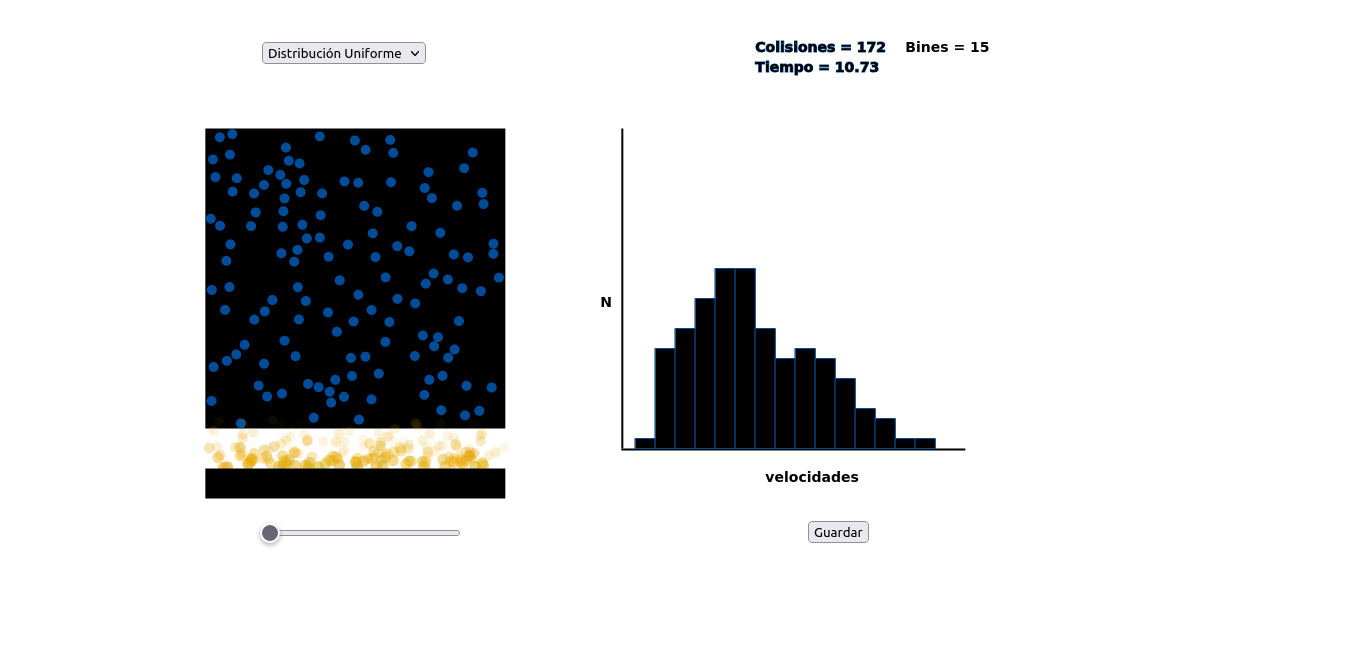
\includegraphics[scale=0.5]{interfaz.png}}
\end{figure}

A continuación se explicará los diferentes elementos en pantalla y el uso de cada uno de los elementos interactivos con los que el usuario puede jugar.

\subsection{Contenedor gas ideal}
\begin{figure}[H]
\centerline{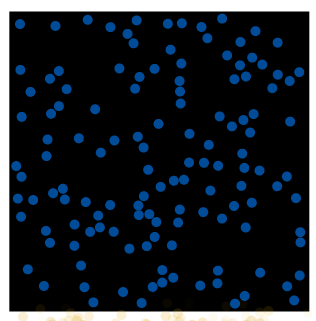
\includegraphics[scale=0.6]{contenedor.png}}
\end{figure}

Están contenidas las partículas con las que se modela el gas ideal y se puede observar su dinámica a lo largo de la simulación, permitiendo visualizar las múltiples colisiones entre las partículas y  de las partículas con las paredes del contenedor. 

\subsection{Histograma de velocidades}
\begin{figure}[H]
\centerline{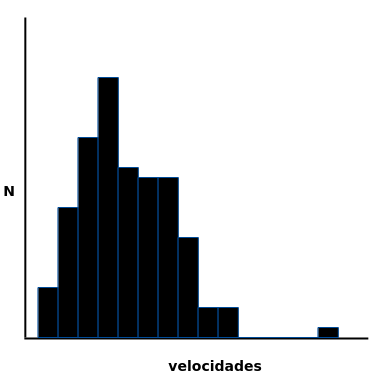
\includegraphics[scale=0.6]{histograma.png}}
\end{figure}

Permite visualizar la distribución de velocidades de las partículas del gas ideal mediante un histograma. Cada bin en el eje horizontal representa un rango de velocidades para las partículas y el eje vertical representa el número de partículas que contiene cada bin del histograma. Es importante resaltar que las velocidades son adimensionales.


\subsection{Panel de información}
\begin{figure}[H]
\centerline{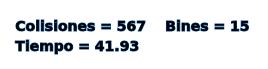
\includegraphics[scale=0.6]{informacion.png}}
\end{figure}

Permite observar en tiempo real información sobre la simulación del gas ideal, tenemos el número de colisiones desde que se inicia la simulación, el tiempo transcurrido desde el inicio de la simulación y el número de bines (grupos) en los que se agrupan las velocidades de las partículas. Hay que tener en cuenta que por inicio de simulación se entiende correr la simulación por primera vez, o cambiar los parámetros de temperatura y/o la distribución que seguirán las velocidades iniciales de las partículas; esto se explicará con más detalle a continuación.

\subsection{Selector de distribuciones de velocidades iniciales}
\begin{figure}[H]
\centerline{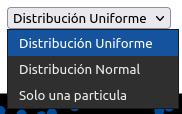
\includegraphics[scale=0.6]{distribuciones.jpeg}}
\end{figure}

En este panel de selección podemos elegir entre tres maneras diferentes de inicializar las velocidades de las partículas del gas ideal:
\begin{itemize}
    \item \textbf{Distribución uniforme:} Con esta opción todas las partículas iniciarán con velocidades aleatorias que siguen una función de distribución uniforme.
    
    \item \textbf{Distribución Normal:} Con esta opción las partículas iniciarán con velocidades aleatorias que siguen una función de distribución normal.
    
    \item \textbf{Solo una partícula:} Con esta opción las partículas iniciarán en reposo y solo una partícula iniciará con una velocidad predefinida según la temperatura del gas.
    
\end{itemize}

\subsection{Fogón}
\begin{figure}[H]
\centerline{
\includegraphics[scale=0.6]{fogon.png}}
\end{figure}

El fogón nos permite variar la temperatura del gas ideal moviendo el botón deslizante a derecha o izquierda, aumentando o disminuyendo la temperatura respectivamente, haciendo que en promedio las partículas inicien con velocidades mayores o menores según la posición de temperatura elegida. Esto es de manera cualitativa, es decir, cuando se desliza el botón, se aumenta o disminuye el valor de las velocidades iniciales, pero no se usa una expresión de temperatura estrictamente.

\subsection{Botón guardar}
\begin{figure}[H]
\centerline{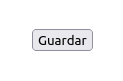
\includegraphics[scale=0.6]{boton.png}}
\end{figure}

Presionando este botón se guardan las velocidades de las partículas en el instante en que se presiona y se descarga un archivo \textit{output.txt} en la ubicación predefinida por el sistema para las descargas. Con estos archivos se realizarán las actividades propuestas explicadas a continuación.

\begin{figure}[H]
\centerline{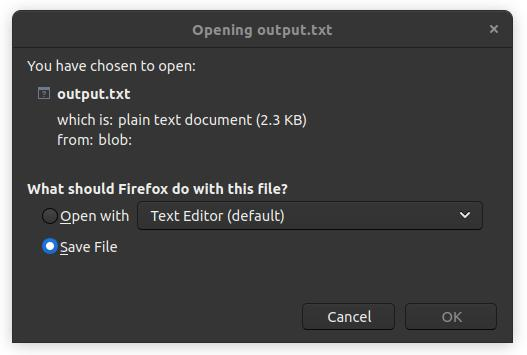
\includegraphics[scale=0.6]{guardar.jpeg}}
\end{figure}


\section{Actividades propuestas}

El fin de las actividades es observar el comportamiento de la distribución de velocidades después de muchas colisiones partiendo de diferentes parámetros de temperatura y velocidades iniciales, por ende las siguientes actividades serán un poco repetitivas para que al final en retrospectiva se pueda observar y entender con mayor claridad el fenómeno físico y la estadística propia de este.  

\subsection{}
Seleccione en el selector de distribuciones la distribución uniforme y en el fogón la temperatura más baja; guarde los datos después de 20 colisiones, grafique estos en Python y ajústelos a la distribución más adecuada según la teoría vista. Deje que transcurran 800 colisiones, descargue los datos y ajústelos a la distribución más adecuada. Repita lo anterior después de transcurridas 1500 colisiones.  

\subsection{}
Seleccione en el selector de distribuciones la distribución uniforme y en el fogón una temperatura de la mitad; guarde los datos después de 50 colisiones, grafique estos en Python y ajústelos a la distribución más adecuada según la teoría vista. Deje que transcurran 800 colisiones, descargue los datos y ajústelos a la distribución más adecuada. Repita lo anterior después de transcurridas 1600

\subsection{}
Seleccione en el selector de distribuciones la distribución uniforme y en el fogón la temperatura más alta; guarde los datos después de 100 colisiones grafíquelos en Python y ajústelos a la distribución más adecuada según la teoría vista. Deje que transcurran 800 colisiones, descargue los datos y ajústelos a la distribución más adecuada. Repita lo anterior después de transcurridas 1600

\subsection{}
Seleccione en el selector de distribuciones la distribución normal y en el fogón la temperatura más baja; guarde los datos después de 20 colisiones grafíquelos en Python y ajústelos a la distribución más adecuada según la teoría vista. Deje que transcurran 800 colisiones, descargue los datos y ajústelos a la distribución más adecuada. Repita lo anterior después de transcurridas 1000

\subsection{}
Seleccione en el selector de distribuciones la distribución normal y en el fogón una temperatura de la mitad; guarde los datos después de 50 colisiones grafíquelos en Python y ajústelos a la distribución más adecuada según la teoría vista. Deje que transcurran 500 colisiones, descargue los datos y ajústelos a la distribución más adecuada. Repita lo anterior después de transcurridas 1000

\subsection{}
Seleccione en el selector de distribuciones la distribución normal y en el fogón una temperatura más alta; guarde los datos después de 100 colisiones grafíquelos en Python y ajústelos a la distribución más adecuada según la teoría vista. Deje que transcurran 500 colisiones, descargue los datos y ajústelos a la distribución más adecuada. Repita lo anterior después de transcurridas 1000

\subsection{}
Seleccione en el selector de distribuciones una sola partícula y en el fogón la temperatura más baja; guarde los datos después de 200 colisiones grafíquelos en Python y ajústelos a la distribución más adecuada según la teoría vista. Deje que transcurran 400 colisiones, descargue los datos y ajústelos a la distribución más adecuada. Repita lo anterior después de transcurridas 600

\subsection{}
Seleccione en el selector de distribuciones una sola partícula y en el fogón una temperatura de la mitad; guarde los datos después de 200 colisiones grafíquelos en Python y ajústelos a la distribución más adecuada según la teoría vista. Deje que transcurran 400 colisiones, descargue los datos y ajústelos a la distribución más adecuada. Repita lo anterior después de transcurridas 800

\subsection{}
Seleccione en el selector de distribuciones una sola partícula y en el fogón la temperatura máxima; guarde los datos después de 200 colisiones grafíquelos en Python y ajústelos a la distribución más adecuada según la teoría vista. Deje que transcurran 400 colisiones, descargue los datos y ajústelos a la distribución más adecuada. Repita lo anterior después de transcurridas 800

\subsection{Preguntas}

\begin{itemize}
    \item ¿Qué distribución empieza a seguir el modelo de gas ideal cuando iniciamos con velocidades distribuidas uniformemente, si dejamos que transcurran muchas colisiones? ¿Sucede lo mismo para todas las distribuciones? 
    \item ¿Qué sucede cualitativamente con las velocidades cuando se aumenta la temperatura? ¿Cómo puede argumentar lo anterior basado en las gráficas que realizó?
    
\end{itemize}





























\end{document}
